%%%%%%%%%%%%%%%%%%%%
\chapter{Results} \label{sec:evaluation}
%%%%%%%%%%%%%%%%%%%%

This chapter describes the experiments with the methodology in Chapter~\ref{sec:methodology}. We begin by examining the IO-Constraint prediction model. We show that a prediction model can be trained using this IO method, but its performance is no better than ordinary linear regression. We also test reweighting the training examples in the loss function. On a small ND problem, we first show that regret improves when setting the weight manually, and then test the performance of the iterative weight update method.

\section{Evaluating \textit{IO-constraint}} \label{sec:eval:io-constraint}

We evaluate \textit{IO-constraint} on two experiments that use synthetic data. The first experiment is a simple two-commodity ND problem with uncertain demands, where we demonstrate that \textit{IO-constraint} can train a linear prediction model. The second example compares the performance of \textit{IO-constraint} with that of a standard linear regression model on a ND problem where the demand is very close to the arc capacity. We also outline the data generation process for the training and test datasets that is common to both examples.

\subsection{Data Generation}

Both experiments rely on synthetic datasets for training and evaluation.  An experiment is defined on a MCFND problem instance in which the demand is uncertain. Our procedure generates can generate a training and test dataset. Each point in the dataset contains the contextual information: $\phib \in \mathbb{R}^m$, the actual demands $\db = [d^1\, \ldots \, d^{|\mathcal{K}|}]^\top \in \mathbb{R}^{|\mathcal{K}|}$, and the optimal solution to the MCFND for those demands: $x^*(\db), y^*(\db)$

Our procedure generates a dataset of $L$ training points $\mathcal{D} = \{(\phib_l, \db_l, x^*(\db_l), y^*(\db_l))\}^L_{l=1}$ which we split into a training and test set $\mathcal{D} = \mathcal{D}_\text{train} \cup \mathcal{D}_\text{test}$.

In our experiments, we assume the demands are a linear function of the contextual information with added Gaussian noise. Given contextual information $\phib \in \mathbb{R}^m$, a vector $\theta_k \in \mathbb{R}^m$ and the noise standard deviation $\sigma_k$, we can express the demand for commodity $k$ as follows:
\begin{align}
    d^k = \theta_k^\top \phib + \epsilon^k \qquad\qquad\text{with}\quad \epsilon^k \sim \mathcal{N}(0, \sigma_k^2).
\end{align}

In our experiments, we wish to generate a dataset of context  such that the expected value of the demand is some fixed value $B_k = \mathbb{E}[d^k] \in \mathbb{R}$. Since there are $m$ points of contextual information and we assume that $m \geq |\mathcal{K}|$, we can randomly generate $m - |\mathcal{K}|$ components of $\phib$ and compute the remaining $|\mathcal{K}|$ components. Given fixed weights $\theta_1, \ldots, \theta_{|\mathcal{K}|}$, we generate each point $(\phib, \db, x^*(\db), y^*(\db)$ in the dataset using the following procedure:
\begin{algorithm}
    \caption{Data generation}\label{alg:eval:data-gen}
    \DontPrintSemicolon
    \SetKwInOut{Input}{Input}\SetKwInOut{Output}{Output}

    \KwIn{number of points $N$}
    \AlignedKwIn{target expected demands $B_k$ and variances $\sigma_k$}
    \AlignedKwIn{demand generation weights $\theta_1, \ldots, \theta_{|\mathcal{K}|}$}
    \AlignedKwIn{contextual information bounds $a,b \in \mathbb{R}$}
    \KwOut{Datasets $\mathcal{D}_\text{train}$, $\mathcal{D}_\text{train}$}
    
    \BlankLine
    \nl Create empty dataset $\mathcal{D}$\;

    \For{i = 1, \ldots, N}{
    \nl Draw $\phi_1, \ldots, \phi_{m - |\mathcal{K}|} \sim U(a,b)$\;
    \nl Set $\phi_{m - |\mathcal{K}| + 1}, \ldots, \phi_m$ by solving $B_k = \theta_k \phib$ for all $k$\;
    \nl Draw noises $\epsilon^k \sim \mathcal{N}(0, \sigma_k^2)$ for all $k$\;
    \nl Solve MCFND($\db$) to get $x^*(\db), y^*(\db)$\;
    \nl Add sample $(\phib, \db, x^*(\db), y^*(\db)$ to $\mathcal{D}$\;
    }

    \nl Separate $\mathcal{D}$ into $\mathcal{D}_\text{train}$ and $\mathcal{D}_\text{test}$ using a random 70\%-30\% split\;
    \nl Return $\mathcal{D}_\text{train}$, $\mathcal{D}_\text{test}$\;
\end{algorithm}

% ==============================================================

\subsection{First Experiment: Training a Prediction Model with IO-Constraint} \label{sec:eval:io-constraint-first-experiment}

This experiment tests whether \textit{IO-constraint} is capable of training a linear prediction model that predicts commodity demands from contextual information. We test the method on a MCFND instance with two nodes and two arcs $p$ and $q$ connecting them, as in Example~\ref{exmp:methodology:opti-def}. Arc $p$ has a low design cost but is has a low capacity $u_p = 15$, whereas arc $q$ is not capacity constrained but has a high design and flow cost. Two commodities $k=1$ and $k=2$ flow from node $s$ to $t$. We fix the size of the contextual information vector $m = 3$ and weights $\theta_1, \theta_2$ then generate a training and test set using Algorithm~\ref{alg:eval:data-gen}. We choose the expected value of the demands $B_1$ and $B_2$ such that the sum of both is slightly above arc $p$'s capacity (i.e. $B_1 + B_2 = 16 \geq u_p$) and set a standard deviation of $\sigma_1 = 2.5$ and $\sigma_2 =1.2$. This results in the optimal solution only building arc $p$ in some cases, and building both arcs in others.

The \textit{IO-constraint} model takes in a dataset of contextual information $\phib_l$ and forward solutions $x^*(\db)_l$ and recovers prediction weights $\hat{\Theta} = [\hat{\theta}_1\, \hat{\theta}_2]^\top$. We test the model on training datasets of increasing size and we observe the Frobenius norm of the difference between the predicted weights and the actual weights used to generate the data.
\begin{equation}
    \lVert \hat{\Theta} - \Theta \rVert_F = \sqrt{\sum_{k=1}^{|\mathcal{K}|} \sum_{i=1}^m (\hat{\theta}_{km} - \theta_{km})^2}
\end{equation}
This aims to measure the distance between the recovered weights and the actual weights used to generate the data. As the model and the data generation process are aligned, we expect that the distance between the two weights decreases to zero as the size of the training dataset increases, with a small imprecision due to the added noise in the demands.

\begin{figure}
    \centering
    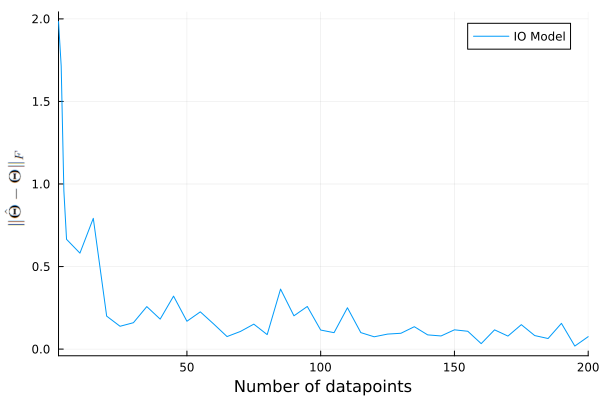
\includegraphics[width=0.6\textwidth]{res/img/frobenius.png}
    \caption{Distance between weights $\hat{\Theta}$ recovered by \textit{IO-constraint} and actual weights $\Theta$ as training dataset size increases.}
    \label{fig:eval:frobenius}
\end{figure}

We see in Figure~\ref{fig:eval:frobenius} that the distance between the weights $\hat{\Theta}$ recovered by \textit{IO-constraint} and the actual weights $\Theta$ decreases to zero as the size of the dataset increases. In particular, the distance is close to zero after $L=25$ points and then hovers slightly above zero. We attribute the remaining difference between the weights to the noise added to the demands in the data generation process. We determine that \textit{IO-constraint} can indeed train a prediction model and recover appropriate weights when the data and the prediction model are aligned.

We have demonstrated in this experiment that it is possible to train a linear prediction model using IO-Constraint, but we have not compared its performance to other models such as standard linear regression. 

% ==============================================================

\subsection{Second Experiment: Comparing \textit{IO-constraint} to Linear Regression}

The second experiment compares the downstream optimization cost of \textit{IO-Constraint} and a linear regression model, on a problem that is designed to highlight a potential advantage of a DFL model. The ND problem is constructed such that a DFL model which is aware of downstream costs would make different predictions compared to a model trained on prediction accuracy. We train an \textit{IO-Constraint} and a linear regression prediction model on the same dataset. We compare the predictions of each model and also compare the resulting downstream cost of each model using the evaluation procedure in Algorithm~\ref{alg:methodology:pipeline-evaluation}.

Our experiment is defined on the network from Example~\ref{exmp:methodology:opti-def} with a dataset of contextual information-demand pairs $\mathcal{D}$. The dataset is composed of two groups of demands of equal size $\mathcal{D}_\text{train} = \mathcal{D}^\text{close} \cup \mathcal{D}^\text{wide}$. Both groups are generated using Algorithm \ref{alg:eval:data-gen}, such that the expected demand of $\mathcal{D}^\text{close}$ is equal to the capacity of the cheapest arc, and the expected demand of $\mathcal{D}^\text{close}$ is well below the capacity of the cheapest arc. We split the dataset into a training and test dataset.

\begin{figure}[h]
    \centering
    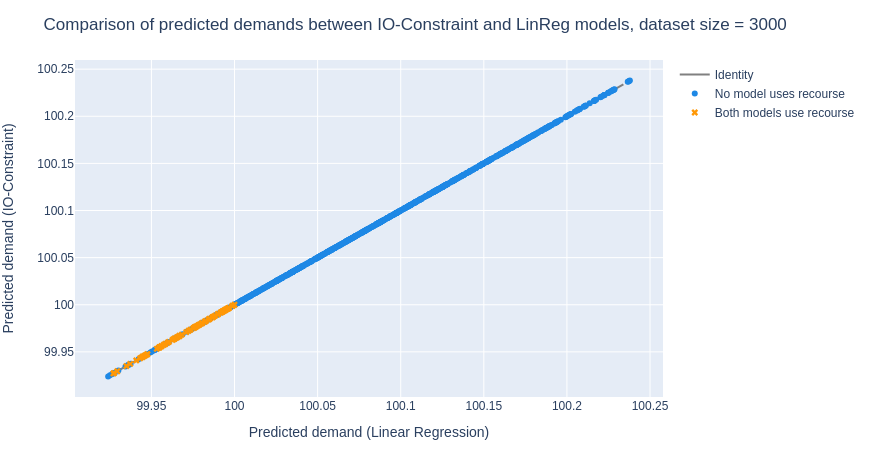
\includegraphics[width=0.7\textwidth]{res/img/pred_comparison.png}
    \caption{Comparison of predictions made by IO-Constraint and a linear regression model. Both models make the same prediction given the same input.}
    \label{fig:eval:pred-comparison}
\end{figure}

We expect a prediction model trained on prediction accuracy to predict values in-between the expected demand of $\mathcal{D}^\text{close}$ and the expected value of $\mathcal{D}^\text{wide}$, whereas we expect a DFL prediction model trained on downstream cost to predict close to the expected value of $\mathcal{D}^\text{close}$, since DFL lends more weight to the solutions that strongly affect decision cost. 

\begin{figure}[ht]
    \centering
    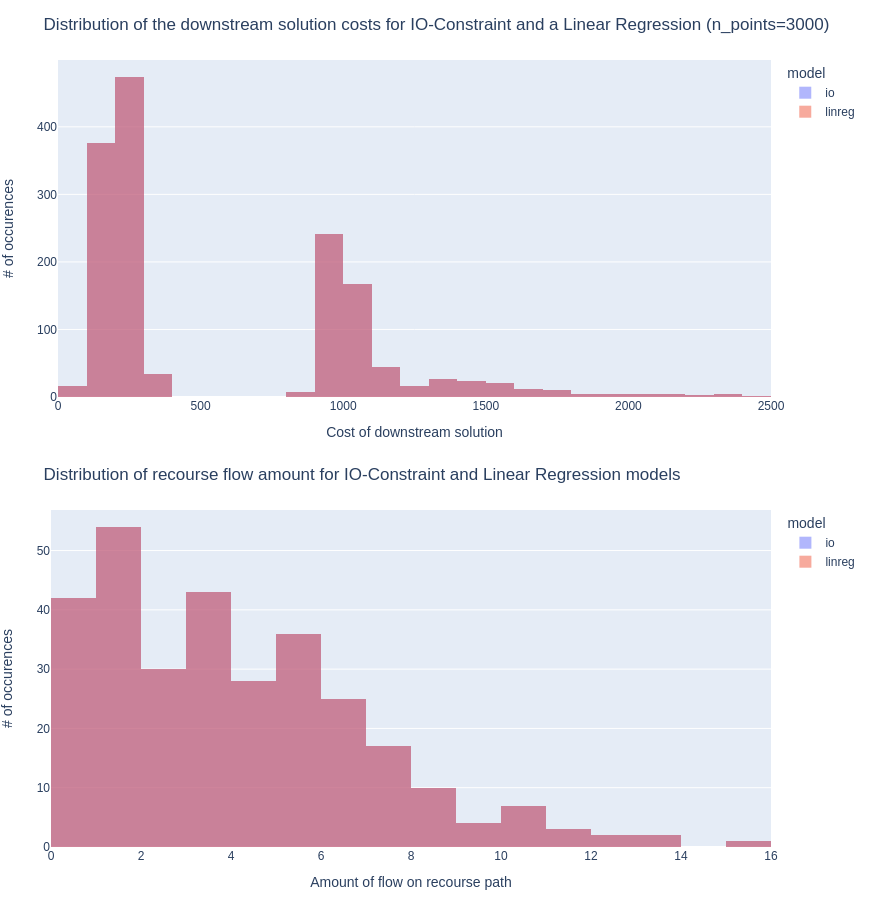
\includegraphics[width=0.7\textwidth]{res/img/dist_flow_costs.png}
    \caption{Distributions of the costs of the downstream solution (top) and of the amount of flow on the recourse arcs (bottom) for \textit{IO-Constraint} and a linear regression model. The distributions of both models are identical.}
    \label{fig:eval:dist-flow-costs}
\end{figure}

We evaluate two linear regression models: an Ordinary Least Squares (OLS) regression model and \textit{IO-Constraint}. We compare the values of the demand prediction made by each model in Figure~\ref{fig:eval:pred-comparison}, and the distribution of downstream cost and flow on the recourse arcs used for each model in Figure~\ref{fig:eval:dist-flow-costs}. As we can see in both figures, both models have the same downstream cost and even produce the exact same prediction given the same contextual information on the test set. 

Our experiment thus confirms our idea that a prediction model trained with \textit{IO-Constraint} corresponds to OLS regression. It does not perform DFL and more work is needed to improve the downstream cost of predictions. 



% ==============================================================
% ==============================================================
% ==============================================================

\section{Reweighting Training Examples with a Misspecified Model} \label{sec:eval:reweighting}

This experiment showcases the utility of reweighting the training examples in the training phase discussed in Section~\ref{sec:methodology:weightings}. In this section, we show a way to improve the downstream cost of a linear predictive on a small ND problem. We use a linear regression model and change the weighting of the training examples in the loss function, treating the weighting as a hyperparameter of the model. By weighting training samples that strongly impact downstream optimization more heavily, we improve the performance of the predictive model once training is over, even though the prediction model is misspecified with respect to the data.

Consider a MCFND problem with three nodes $\mathcal{N} = \{A,B,C\}$, three arcs $\mathcal{A} = \{AB, AC, CB\}$, and two commodities $k=1$ and $k=2$.

\begin{minipage}{0.45\textwidth}
    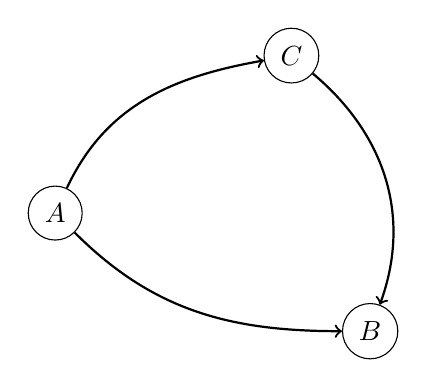
\begin{tikzpicture}[main/.style={draw, circle}]
    \node[main] at (0, 1) (A) {$A$};
    \node[main] at (4, -0.5) (B) {$B$};
    \node[main] at (3, 3) (C) {$C$};

    \draw[->, thick] (A) to [out=65, in=190] (C);
    \draw[->, thick] (A) to [out=-45, in=180] (B);
    \draw[->, thick] (C) to [out=-40, in=70] (B);
\end{tikzpicture}
\end{minipage}
\begin{minipage}{0.45\textwidth}
    Commodity $k=1$ originates in $A$ and flows to $B$ with demand $d^1$. Commodity $k=2$ also originates in $A$ and goes $C$ with demand $d^2$. 

    Arc capacity is almost equal to demand on arc $AB$ and is much higher than demand on arcs $AC$ and $CB$: $u_{AB} \approx d^1$ and $u_{AC}, u_{CB} \gg d^1 + d^2$.
\end{minipage}

Flow costs are zero $c_{ij}^k = 0$ for all arcs and commodities and design costs are equal $f_{AB} = f_{AC} = f_{CB} = F$. 

Suppose the demands are generated from the same contextual information $\phi \in  \mathbb{R}$ using two different linear functions with added noise:
\begin{equation}
\begin{aligned}
    d^1 &= \theta^\mathrm{int}_1 + \theta_1\phi + \epsilon^1\\
    d^2 &= \theta^\mathrm{int}_2 + \theta_2\phi + \epsilon^2
\end{aligned}
\end{equation}
where $\theta^\mathrm{int}_1$ and $\theta^\mathrm{int}_2$ are the intercepts, $\theta_1$ and $\theta_2$ the slopes, $\epsilon^1, \epsilon^2 \sim \mathcal{N}(0, \sigma^2)$ the independently-drawn Gaussian noise for each respective commodity. The parameters are select such that the expected value of the demand for commodity $k=2$ is very close to the capacity of arc $AB$, i.e. $\mathbb{E}[d^2] \approx u_{AB}$.

Now consider a misspecified linear prediction model $f_{\theta^\text{int},\theta}$, which predicts each commodity with two different intercepts $\theta^\mathrm{int}_1$ and $\theta^\mathrm{int}_2$ but the same slope $\theta \in \mathbb{R}$:
\begin{equation}
\begin{aligned}
    \hat{d}^1 &= f_{\theta^\mathrm{int}_1, \theta}(\phib) = \theta^\mathrm{int}_1 + \theta \phib\\
    \hat{d}^2 &= f_{\theta^\mathrm{int}_2, \theta}(\phib) = \theta^\mathrm{int}_2 + \theta \phib
\end{aligned}
\end{equation}
The prediction model is trained over a dataset of contextual info and demand pairs. The dataset is comprised of samples from the distribution of commodity $1$ and commodity $2$: $\mathcal{D}_\mathrm{train} = \mathcal{D}_\mathrm{train}^1 \cup \mathcal{D}_\mathrm{train}^2 = \{(\phi_i, d_i, k_i)\}_{i=1}^N$, where $k_i$ indicates which commodity the training sample refers to. 

Looking closely at this example, we see that accurately predicting demand $d^1$  is much more important than predicting demand $d^2$. Because $d^1$ is so close to the capacity of arc $AB$, overprediction results in both arcs $AB$ and $CB$ being built, even though arc $AB$ would have been sufficient. This increases the cost of the final downstream optimization problem from $2F$ to $3F$. Because the demand $d^2$ is so far from the capacity of arc $AC$, the prediction error of $d^2$ has no effect on which arcs are built.

\begin{figure}
    \centering
    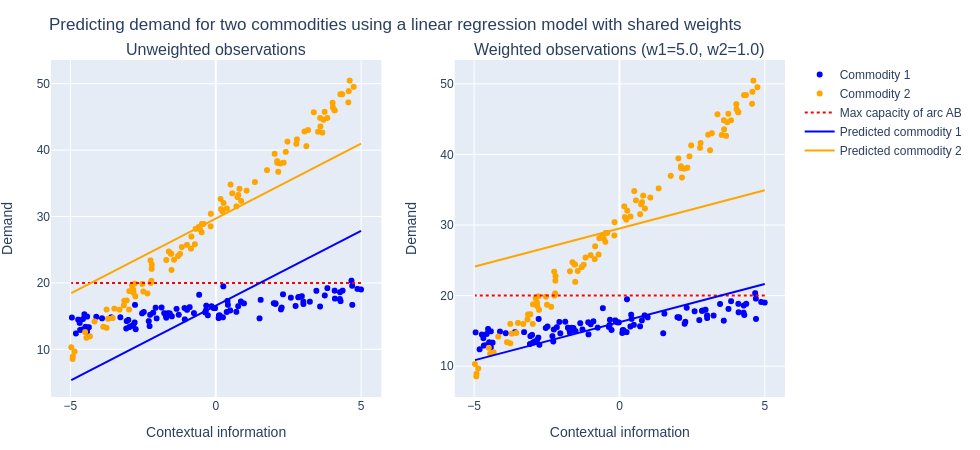
\includegraphics[width=\textwidth]{res/img/metho-weightings.png}
    \caption{Comparison of linear regression with unweighted and weighted training examples. The weighted model has worse prediction performance but lower downstream optimization cost overall.}
    \label{fig:eval:weightings-graph}
\end{figure}

Figure \ref{fig:eval:weightings-graph} illustrates the example with an arc cost of $F=1$, and compares two linear regression prediction models defined above. Despite having a higher overall prediction error, the weighted model predicts demands that result in lower downstream optimization costs and regret, as shown in Table~\ref{tab:eval:weighting-results}. In the unweighted case, each training sample is equally weighted in the model's loss function. A prediction error for commodity 1 will have the same effect on the model as a the same prediction error for commodity 2. The slope of the unweighted prediction model lands halfway in-between the two commodities. In the weighted case, the training samples from commodity 1 are weighted 5 times more than those from commodity 2. This results in a flatter slope, much closer to the slope of commodity 1. The unweighted model predicts a demand for commodity 1 that is above the arc capacity of $AB$ much more often than the weighted model.

\begin{table}[h]
    \centering
    \begin{tabular}{ l l l l } 
    \hline
    Model &  RMSE & Optim. cost & Regret \\
    \hline
    Unweighted & \textbf{5.19} & 1.15 & 0.15\\ 
    Weighted & 6.18 & \textbf{1.07} & \textbf{0.07}\\
    \hline
    \end{tabular}
    \caption{Caption}
    \label{tab:eval:weighting-results}
\end{table}

\section{Iterative Search for Training Example Weightings} \label{sec:eval:iterative}

In this experiment, we test the iterative weight update method devised in Section~\ref{sec:methodology:weightings}. Having shown in Section~\ref{sec:eval:reweighting} above that reweighting the training examples can lead to better downstream performance, we test a systematic way to find a weighting of the training examples that improves downstream performance. This corresponds to finding a solution for the W-DFL problem defined in (\ref{eq:methodology:w-dfl}) using the iterative weight update from (\ref{eq:methodology:update-weights-prop}) and (\ref{eq:methodology:update-weights-norm}). We use the same ND example problem and experimental setup as in Section~\ref{sec:eval:reweighting}. We set the flow cost of the recourse arcs in MCFND-Flow to $c_\text{rec} = 10$ to cover the case where the demand is higher than the capacity of arc $AB$, but the model predicts a demand below the capacity. We generate a second dataset $\mathcal{D}_\text{test}$ using the method as $\mathcal{D}_\text{train}$ to evaluate the regret of the prediction model on unseen data. Starting with all training examples weighted equally at iteration $t=1$, we update the weightings until $t=1200$ iterations. 

The iterative method improves regret on this example up to a certain point, after which regret increases dramatically. Figure \ref{fig:eval:iterative-regret} shows the evolution of regret at every iteration, on both the training dataset $\mathcal{D}_\text{train}$ and the test dataset $\mathcal{D}_\text{test}$. It shows that regret steadily decreases with the number of iterations, from an initial test regret of 28 when all observations are weighted equally, to the minimum test regret of 1.22 starting at iteration $t=538$. However, as the number of iterations increases past $t=700$, the regret starts to rise. Finally, after $t=1057$, the regret oscillates in an unstable manner between a high value of 100 and a lower value around 20. This is a phenomenon specific to our example, where the only examples contributing to regret after enough iterations are those with a demand above the capacity of arc $AB$. Those examples become very heavily weighted, causing all the other predictions to be above the arc capacity and thus increasing regret for all training examples drastically. 

\begin{figure}
    \centering
    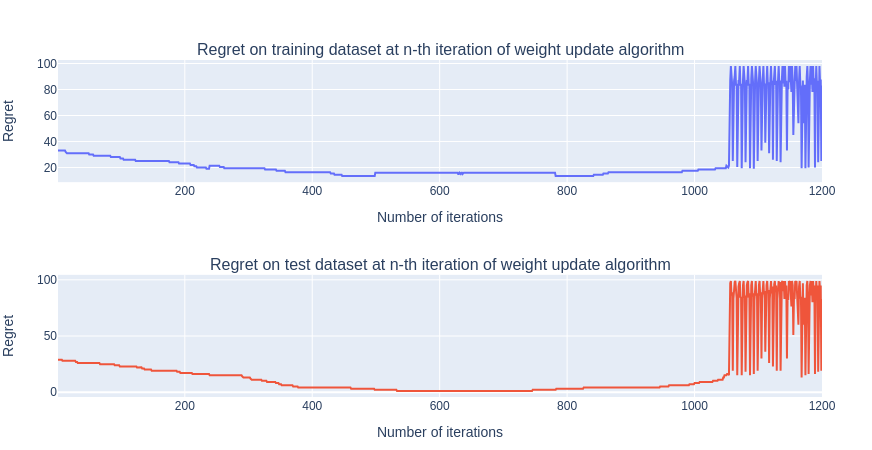
\includegraphics[width=\textwidth]{res/img/iterative.png}
    \caption{Progression of training and test regret at every iteration of the weight update algorithm.}
    \label{fig:eval:iterative-regret}
\end{figure}

This experiment shows the promise of a iterative weight update method for solving the W-DFL problem. The method yields weightings that improve downstream optimization cost on a small example. However, without a theoretical backing, this behaviour could be limited to this small example. This method also seems to present instability after a sufficient number of iterations. Perhaps a better weight update rule or stopping criterion could further improve the performance of the iterative method.

%In the evaluation you convince the reader that your design works as intended.
%Describe the evaluation setup, the designed experiments, and how the
%experiments showcase the individual points you want to prove.

%This section is usually 5-10 pages.
